\documentclass[FM,RP]{tulthesis}
\usepackage{tul}
\usepackage[czech]{babel}
\usepackage[utf8]{inputenc}
\usepackage[LY1,T1]{fontenc}
\usepackage[utf8]{inputenx}
\usepackage[nottoc]{tocbibind}
\usepackage{graphicx}
\usepackage{parskip}
\usepackage{subfig}
\usepackage{xparse,newunicodechar}

\TULtitle{Měření spotřeby elektrické energie na svítidle řízeném protokolem DALI}{Measurement of power consumption on the light fitting controlled by DALI protocol}
\TULprogramme{B 2646}{Informační technologie}{Information technology}
\TULbranch{1802R007}{Informační technologie}{Information technology}
\TULauthor{Lukáš Souček}
\TULsupervisor{Ing. Martin Černík Ph.D.}
\TULyear{2017}
\begin{document}

\ThesisStart{male}
\begin{abstractCZ}
Bakalářský projekt se zabývá zjišťováním spotřeby elektrické energie na jednom konkrétním zařízení.
Mimo jiné se zabývá i možnostmi ovládání světelných systémů a také komunikací se světelnými zařízeními pomocí protokolu DALI v prostředí programu Helvaru Designer spolu s různými nastaveními. Popisuji také i společné součástky a vlastnosti různých protokolů. Je zde zařazeno teoretické seznámení se spotřebou společně s praktickými možnostmi měření spotřeby na svítidle s využitím měřících přístrojů jako je Wattmetr či osciloskop a srovnání s praxí. 
\end{abstractCZ}
\vspace{2cm}
\begin{abstractEN}
		The project report deals with the determination of the consumption of electricity on one particular device. Among other things, it deals with the possibilities of controlling lighting systems as well as communicating with lighting devices using the DALI protocol in the Helvar Designer program environment, along with various settings. I also describe the common components and properties of various protocols. There is a theoretical introduction to consumption together with practical options for measuring luminaire consumption using measuring instruments such as a Wattmeter or oscilloscope and a comparison with practice. 
\end{abstractEN}

\tableofcontents

\clearpage


\begin{abbrList}
   DALI & Digital Addressable Lighting Interface \\
	VA & VoltAmperes \\
    W & Watts \\
    VA & VoltAmperes \\
    V & Volts \\
     A & Amperes \\
\end{abbrList}



\chapter{Úvod}
Tuto práci jsem si vybral za účelem seznámit se s ovládáním světelných zařízení a dozvědět se více o způsobu měření spotřeby, které lze využít nejen u světel, ale i u elektrických zařízení v domácnosti. Vzhledem k tomu, že se s jejich rozvojem zvyšují i nároky na spotřebu elektrické energie, je měření celkové spotřeby aktuálním tématem.

Možnosti jak komunikovat se zařízeními se značně rozšířily, především v oblasti světel, kde je spoustu firem poskytujících zajištění bezproblémového chodu s využitím různých systémů, které chci ve své práci zmínit mimo systém DALI,  který je velkým trendem poslední doby.

Rád bych měřením na světelném zařízení zjistil, jakým způsobem se toto zařízení chová a uvědomil si význam naměřených veličin. Zdokumentováním výsledků bych chtěl potvrdit či vyvrátit domněnky, které z průběhu měření mohou vyplynout.

 
 \chapter {Světelné systémy}
Systémy světel umožňují naší civilizaci zajistit především bezpečnost a možnost regulovat osvětlení dle potřeby. Efektivně lze využít i sjednocení různých systémů dohromady, což je popsáno v podkapitole Ovládání systémů. Kromě toho je také nezbytné nadále rozvíjet možnosti využití dalším rozvojem rozepsaným níže.  
 
 \section{Vývoj světelných systémů}
 Samotné světelné systémy začaly vlastně již s příchodem prvních elektrických lamp v 19. století. Začínaly osvětlovat ulice, a ač ještě neexistovaly žádné počítačové systémy či něco podobného, tak systém pouličního osvětlení byl velký počin pro celé lidstvo. S možností využít co nejvíce potencionál ovládání těchto systémů přišla možnost síťové manipulace ve 20. století za pomoci počítačů, aktuálně také i mobilů a jiných podobných elektronických zařízení.
 \section {Ovládání systémů}
 Síťově ovládané světelné systémy jsou řešením umožňující za pomoci síťového připojení propojit jednotlivá světelná zařízení a jejich ovládací prvky (spínače) v jednotný systém, který pak lze ovládat pomocí určitého protokolu. Toto propojení nám umožní ušetřit elektrickou energii a zároveň zefektivnit ovládání jednotlivých zařízení. Dále tyto systémy poskytují velké množství funkcí jako je regulování osvětlení za pomoci detekce pohybu, plánování intenzity osvětlení dle denní doby či zobrazení informativních statistik osvětlení (výkon, spotřeba).  
 \cite{daintree.net}
 \cite{wiki:Lighting_control_system}
 \newpage
 \section {Protokol DALI}
  Nejvýznamnějším protokolem používaným v této době je DALI. V podstatě se jedná o rozhraní umožňující využít stmívatelných předřadníků od různých výrobců. DALI je zároveň i jednoduchá forma jak komunikovat s různými komponentami v oblasti světelné technologie. Neexistují zde speciální požadavky pro vedení kabeláže datových kabelů, takže není potřeba instalovat omezovací rezistory pro kabely kvůli ochraně před odrazy. S větší flexibilitou a zjednodušením instalace v řadě různých aplikací DALI pomalu nahrazuje Analogové rozhraní 1-10 Voltů, které je aktuálně nejběžnějším standardem pro stmívače elektronických předřadníků.
\cite{DALI-manual}
 
 \section {Ostatní protokoly}
  
  \subsection{KNX}
  KNX protocol se vypořádává s problémy izolování zařízení zajištěním komunikace v jednom společném jazyce. Za pomoci KNX média, ke kterému jsou připojena všechna sběrnicová zařízení si lze vyměňovat různé informace. Sběrnicová zařízení mohou být senzory či akčními členy (aktuátory) potřebné pro řízení zařízení spravující různé funkce budov, např. ventilační systémy, monitorovací systémy či ovládání světel. Všechny tyto funkce můžou být kontrolovány i monitorovány jednotným systémem bez nutnosti potřeby dalšího centra ovládání. \cite{knx-introduction}
  \subsection{0-10 Voltů}
  Jedná se o analogové ovládání pomocí určitého signálu. Protokol 0-10 Voltů jak již název napovídá, aplikuje voltáž mezi nulou a deseti Volty pro ovlivnění intenzity osvětlení. Existují 2 typy standardu ovládání dle tohoto protokolu, první z nich byl používaný pro divadelní osvětlení. Modernější a dodnes používaný typ najde uplatnění u řízení stmívacích předřadníků. Aktuální používaný typ vyžaduje, aby předřadník poskytoval plný výkon světla, pokud bude napětí na maximu.
  Minimum světla, ideálně žádné poskytuje předřadník pokud je napětí 1 volt či méně, tyto vlastnosti minima a maxima se však můžou u každého zařízení lišit. 
  \cite{0-10Volts}
 \newpage
 \section{Společné vlastnosti a součástky protokolů }
 Využití několika vlastností, jako je kupříkladu napájení samotné, je společnou vlastností všech zmíněných protokolů, využívajících elektrickou síť jako zdroj energie. Další společnou vlastností je nahraditelnost protokolů, především u DALI a 0-10 Voltů, které se můžou vyměnit navzájem. S použitím zmíněných protokolů lze využít zařízení jako je Dimmer či Ballast popsané níže, která umožňují efektivní a užitečnou komunikaci s dalšími světelnými zařízeními. 
  
  \subsection{Dimmer}
  Součástka dimmer je stmívač ukrytý zpravidla pod krytem určitého spínače ovládajícího světlo. Světelný stmívač pracuje v podstatě tím, že vysekne části ze střídavého napětí. To umožňuje přenášet pouze části křivky na lampu či žárovku. Čím více takovýchto nasekaných křivek, tím větší jas. Pokud se na takovéto části  podíváme, uvidíme písmeno zploštělé písmeno s, viz. obr. \ref{osekanakrivka}.
  Původní neosekaná křivka je na obr. \ref{sinusovakrivka}.  
  
  
  Existují zpravidla 2 typy stmívačů. Dříve se využíval typ, který měl v sobě rezistor nebo velký transformátor. Tento stmívač měl ručně ovládané kolečko nastavující úroveň výstupu, viz obr. \ref{dimmerotocny}. Byl však velmi neefektivní - drahý a velký zároveň. Moderní stmívače mající v sobě triak a tyristor se pouze zapnou či vypnou, a proto nemají takovou spotřebu, jsou kompaktnější a levnější.
    \vspace{2em}
   \begin{figure}[h]
   	\begin{center}
   		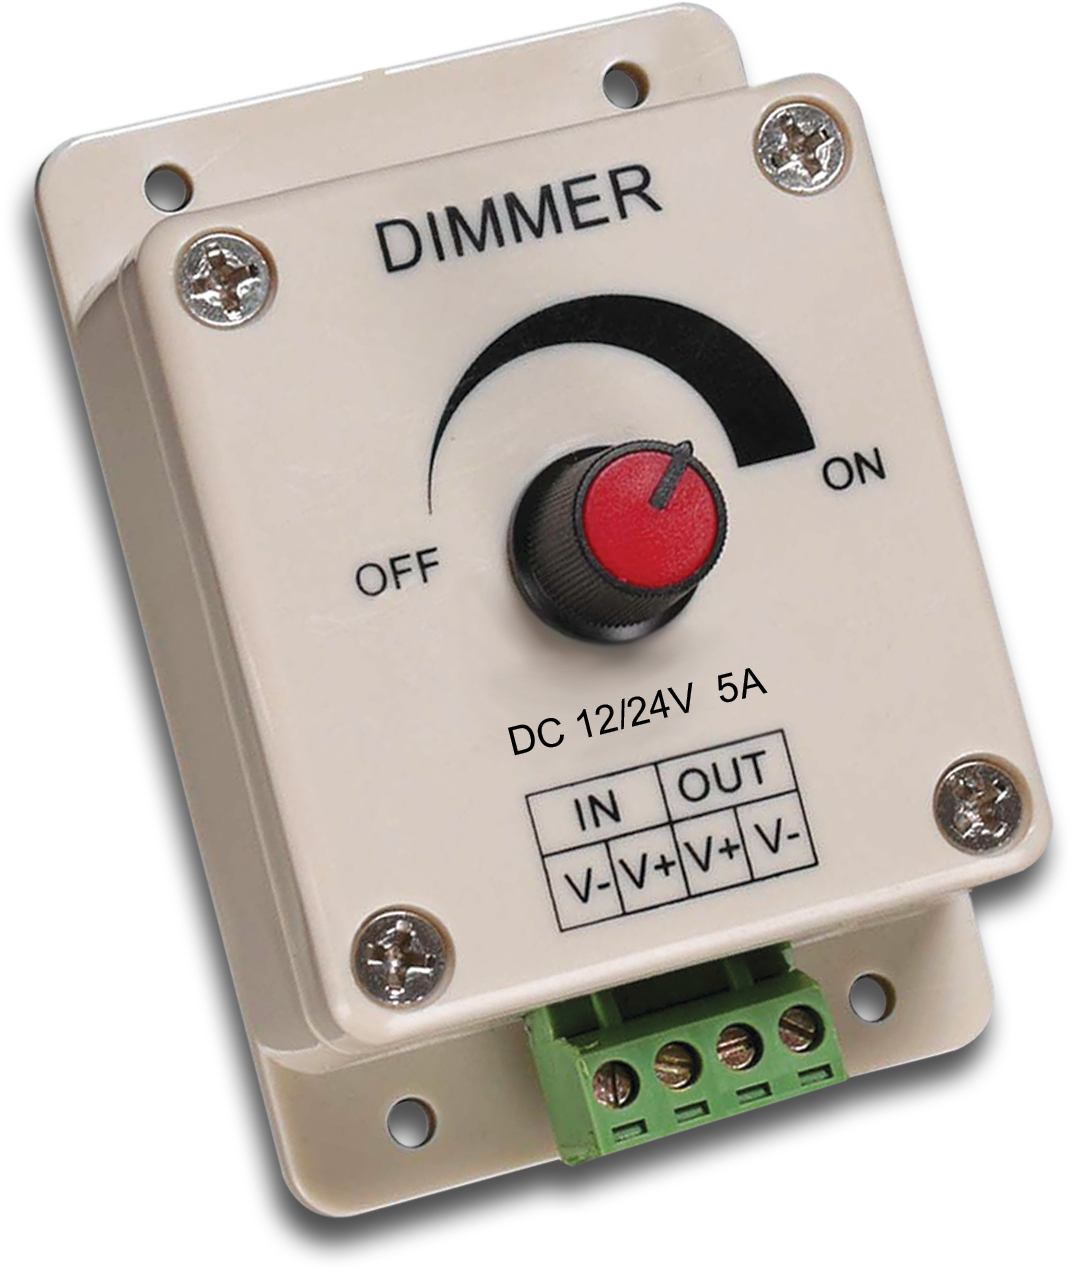
\includegraphics[scale=0.15]{Dimmer-1224-Volt1.jpg}
   		\caption{Otočný stmívač}
   		\label{dimmerotocny}
   	\end{center}
   \end{figure}
   \newpage
    
     
   
  \subsection{Předřadník}
  Předřadník má zpravidla 2 hlavní funkce. Jednou z nich je zapnutí daného spotřebiče, využívá se toho především u zářivek, kde jsou trubice - výbojky, které mají v sobě stlačené plyny. Druhou funkcí je ovládání operací, které se můžou vykonat, jako je zhasnutí, rozsvícení či plánování kdy bude dané svítidlo svítit a jak dlouho. Dříve se využívalo magnetických předřadníků. Princip byl celkem jednoduchý, proud probíhal skrz cívky měděného drátu, po vystavení mědi tomuto proudu se vytvořilo magnetické pole, zachytávající většinu proudu proudícímu k žárovce, tímto způsobem se regulovalo osvětlení.
    
  Avšak s nástupem elektronických předřadníků, které jsou v současné době hojně využívané se magnetické staly pouhou vzpomínkou. Nynější předřadníky mění tok elektřiny za pomocí cívek v sérii, oddělených od sebe. 
  Zároveň cívky mění frekvenci elektrického proudu bez změny napětí. To umožňuje kmitání takovou rychlostí, že žárovky neblikají, na rozdíl od magnetických předřadníků, kde frekvence byla omezená přibližně na 60 Hz, což občas způsobovalo blikání a i bzučení žárovek. Elektronický předřadník také umožňuje stmívat světelné zařízení, čímž vlastně částečně nahrazují stmívače. Hlavním rozdílem obou druhů je v efektivitě, elektronické mají schopnost rozsvítit více výkonnější zářivky. Na obr. \ref{predradnik}  lze vidět ukázku předřadníků.
  
   \begin{figure}[h]
  	\begin{center}
  		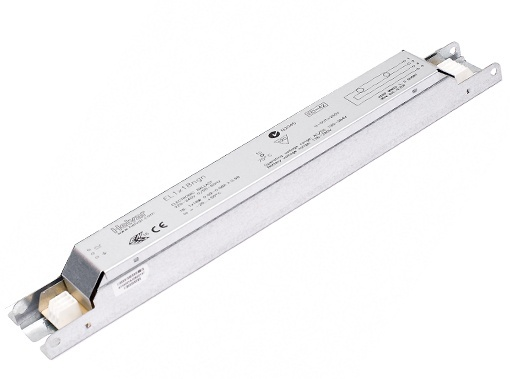
\includegraphics[scale=0.5]{predradnik.jpg}
  		\caption{Předřadník}
  		\label{predradnik}
  	\end{center}
  \end{figure}
  
  
  \begin{figure}[h]
  	\begin{center}
  		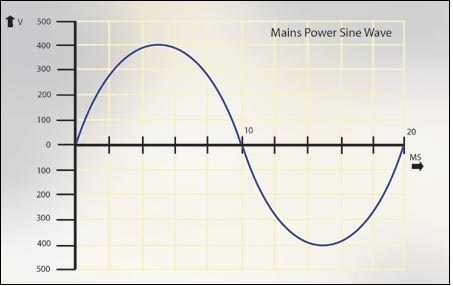
\includegraphics[scale=0.92]{waveform.jpg}
  		\caption{Sinusová křivka}
  		\label{sinusovakrivka}
  	\end{center}
  \end{figure}
  
  
\begin{figure}[h]
	\begin{center}
		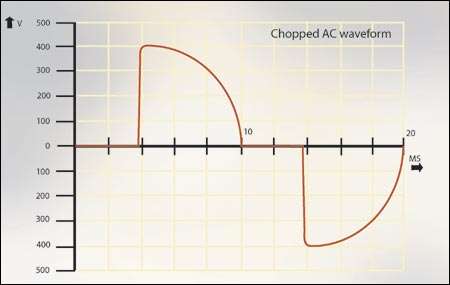
\includegraphics[scale=0.7]{chopped_ac_waveform.jpg}
		\caption{Osekaná sinusová křivka}
		\label{osekanakrivka}
	\end{center}
\end{figure}

 \chapter{Elektrická spotřeba}
   Spotřebovaná energie se využívá v různých odvětvích a jedním z nich je právě elektrická spotřeba. Vyjadřuje, jak moc velkou elektrickou energii využívá dané zařízení za určitou jednotku času. Na obrázku \ref{spotrebaenergie} je vidět ukázka příkonu procesorů v mobilních zařízeních.
   \cite{wiki:Electric_energy_consumption}
   \begin{figure}[h]
   	\begin{center}
   		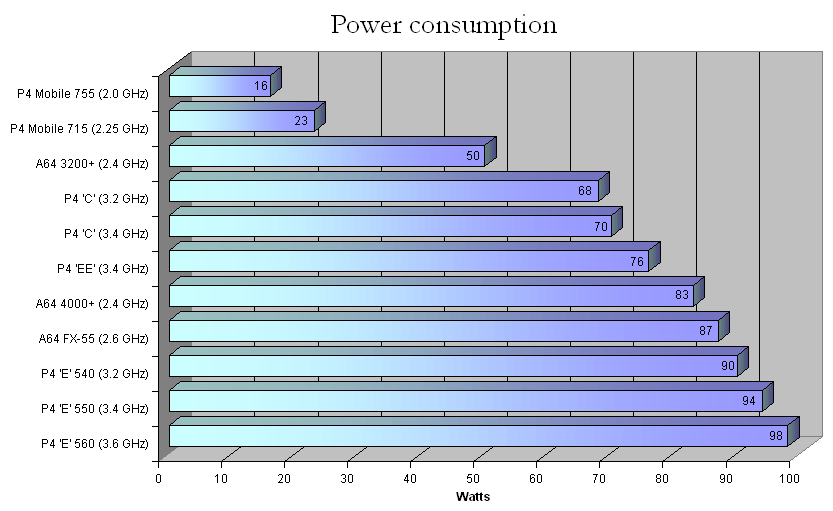
\includegraphics[scale=0.5]{Power_consumption_graph.jpg}
   		\caption{Spotřeba energie mobilních zařízn}
   		\label{spotrebaenergie}
   		\end{center}
   \end{figure}


    \section {Význam}
     Z hlediska zjištění ceny je nezbytné znát, jak velká je spotřebovaná energie ať už se jedná o nějakou společnost či domácnost. Je zároveň druhou nejvyužívanější energií hned po dopravním odvětví. Dále umožňuje statistickému úřadu zjistit spotřebu domácností za rok, aby dodavatelé elektrické energie věděli, zda je možné poskytnout potřebné množství odběratelům.
     \cite{kalkulackaenergie}
   \section {Metody měření}
   Aby se dalo vůbec začít měřit, je třeba znát několik důležitých veličin. Jednou z nich je Příkon (činný výkon), který se měří ve Wattech pomocí Wattmetru. Jelikož se měří činný výkon, který je  elektrickou energií, která se za určitý čas přemění v užitečnou práci a vypočítá se dle vztahu P = U*I*cos $\Phi$, kde U a I jsou efektivní hodnoty napětí a proudu (hodnoty změřené ampérmetrem a voltmetrem) a cos $\Phi$ je účiník určující účinnost přenosu energie ze zdroje střídavého proudu do spotřebiče. 
   
   Vynásobením změřeného proudu i napětí (Pz = U*I). zařízení dostáváme 
   zdánlivý výkon představující výkon, který se dopravuje ke spotřebiči, zdánlivý je proto, že se nezapočítávají ztráty, jeho jednotkou jsou Voltampéry (VA). Posledním výkonem ve střídavých obvodech je jalový výkon - jednotka (VAr) vyjadřující přelévání výkonu tam a zpět, výpočet má podobný jako činný výkon, jen se počítá se sinusovou složkou, pro měření se musí pootočit napětí na napěťové cívce wattmetru. Pro výslednou spotřebu stačí vědět ještě čas, po který je měřené zařízení zapojeno a vynásobením příkonem dostáváme Elektrickou energii E = P*t jejíž jednotkou jsou Watthodiny. 
   
   Dobrý způsob je také specifické změření měřičem spotřeby elektrické energie, který přesně změří spotřebu daného spotřebiče, jediné co stačí je zapojit měřič do zásuvky a následně jakékoliv elektrické zařízení zapojit do něj. Poté by se na displeji měly zobrazit hodnoty spotřeby energie v kilowatech za hodinu a i předpokládané výdaje za spotřebu po dni či měsíci, viz obr. \ref{mericenergie}. \cite{vykon}
    
    \begin{figure}[h]
   	\begin{center}
   		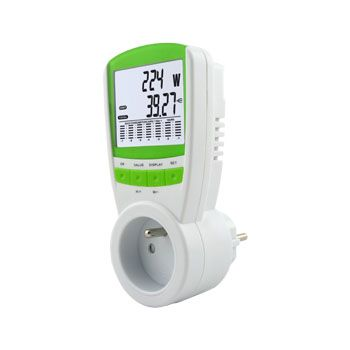
\includegraphics[scale=0.75]{_thb_4731650_obr.jpg}
   		\caption{Měřič spotřeby energie}
   		\label{mericenergie}
   	\end{center}
   \end{figure}
 
   \chapter {Praktická komunikace s DALI}
   V této části kapitoly se zaobírám praktickou manipulací se zařízeními za pomoci protokolu DALI, konkrétně prací v programu pro komunikaci s možností různých nastavení. Tímto se docílí zautomatizování veškerých úkonů, které jsou více než nutné v obrovských prostorách různých firem. Je nezbytné mít v systému router (kontrolní jednotku) umožňující ovládat jak samotná světla, tak ale i celý světelný komplex.
   S touto možností lze samozřejmě z pohodlí domova také ovládat světelný systém, pokud je počítač či notebook připojený kabelem k routeru k internetu, nejen k lokální síti. Na obr. \ref{dalisystem}  lze vidět připojení systému DALI pomocí routeru k počítači - rozhraním Ethernet, struktura je celkem jednoduchá, počítač posílá signál na router a ten ji přeposílá danému zařízení datovými kabely DALI se správnou IP adresou, která je součástí signálu. 
   
   Následně konkrétní zařízení(dimmer, ballast, detektor prezence)  vykoná dle informace co přijde specifickou činnost, v našem případě není zapojena druhá linka DALI 2 pro připojení dalších zařízení při překročení kapacity u DALI 1. Pokud chceme využít více routerů pro ovládání obrovského množství světelných prvků, je třeba nejdříve připojit počítač ke switchi, který zajistí komunikaci mezi více kontrolními jednotkami a počítačem. 
      \section{Prostředí pro práci}
    Před seznamováním se s prostředím, ve kterém jsem začínal pracovat se muselo zkontrolovat propojení se systémem DALI, aby byla zajištěna funkčnost komunikace mezi PC a zařízeními. Abych se vůbec dostal k nastavování jednotlivých komponent muselo se zadat bezpečnostní heslo nutné pro editaci nastavení zařízení a nejen zobrazování jejich vlastností. Hned na úvodní obrazovce mě udivila komplexnost tohoto programu, viz obr \ref{helvardesign}, který není jen pro klasické stmívání, ač jsem si myslel původně něco jiného. Samotná grafická stránka programu je uživatelsky příjemná a vcelku jednoduchá. Seznam zařízeních zobrazených v okně Devices zobrazuje nejprve samotný a k němu přiřazená jednotlivá světelná zařízení, v tomto případě, jak lze vidět z obrázku \ref{helvardesign} 2 zařízení každé s rozdílnou IP adresou pro jednoznačnou identifikaci, nejprve ballast zajišťující regulování zářivek a také detektor pohybu, to vše je zapojeno v jedné podsíti, zatímco malá LED žárovka je v druhém. S každým zařízením lze nadále pracovat dle možností funkcí, které poskytují. 
    \vspace{5em}
      \begin{figure}[h]
    	\begin{center}
    		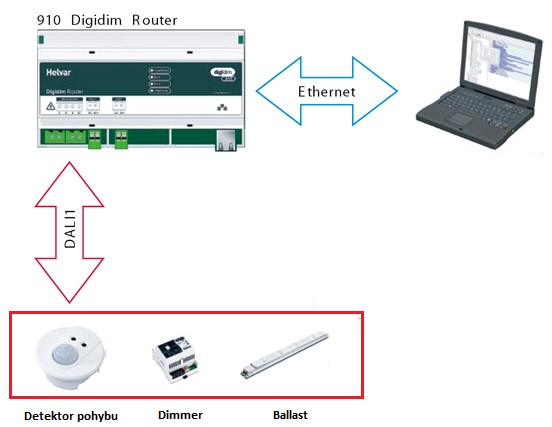
\includegraphics[scale=0.7]{dalisystem.jpg}
    		\caption{Propojení systému DALI}
    		\label{dalisystem}
    	\end{center}
    \end{figure}
\vspace{5
	em}
        \begin{figure}[h]
    	\begin{center}
    				
    		\includegraphics[scale=0.25]{helvar.jpg}
    		\caption{Helvar Designer}
    		\label{helvardesign}
    	\end{center}
        \end{figure}
    \vspace{5em}
    \section{Možnosti nastavení}
    Nastavení v programu Helvar Designer bylo potřeba pečlivě hlídat s ohledem na jednotlivá zařízení, aby nedošlo k případné interferenci mezi nastaveními. Šlo velmi efektivně využít zapnutí světel v určitou dobu, reakce světel byla přibližně okolo jedné sekundy, lehce se také manipulovalo s intenzitou osvětlení pomocí ballastu, které se pak využilo v kapitole měření spotřeby a i při nižším osvětlení byly světelné podmínky dostatečné, rozdíl byl znát až při nějakých 30 procentech výkonu zářivky. 
    
    Sjednocení komponent do jednotlivých skupin bylo jednou z nejlepších možností jak zajistit ovládání více zařízení najednou nastavováním různých scén v dané skupině. Router, se kterým jsem komunikoval lze vidět na obr. \ref{dalisys}, kde je vidět na pravé straně černý kabel jdoucí do napájení a horním otvorem jde propojovací kabel Ethernet napojený do počítače, v levé části lze vidět kabeláž vedoucí k samotným světelným zařízením.
  \vspace{2em}
    \begin{figure}[h]
    	\begin{center}
    		
    		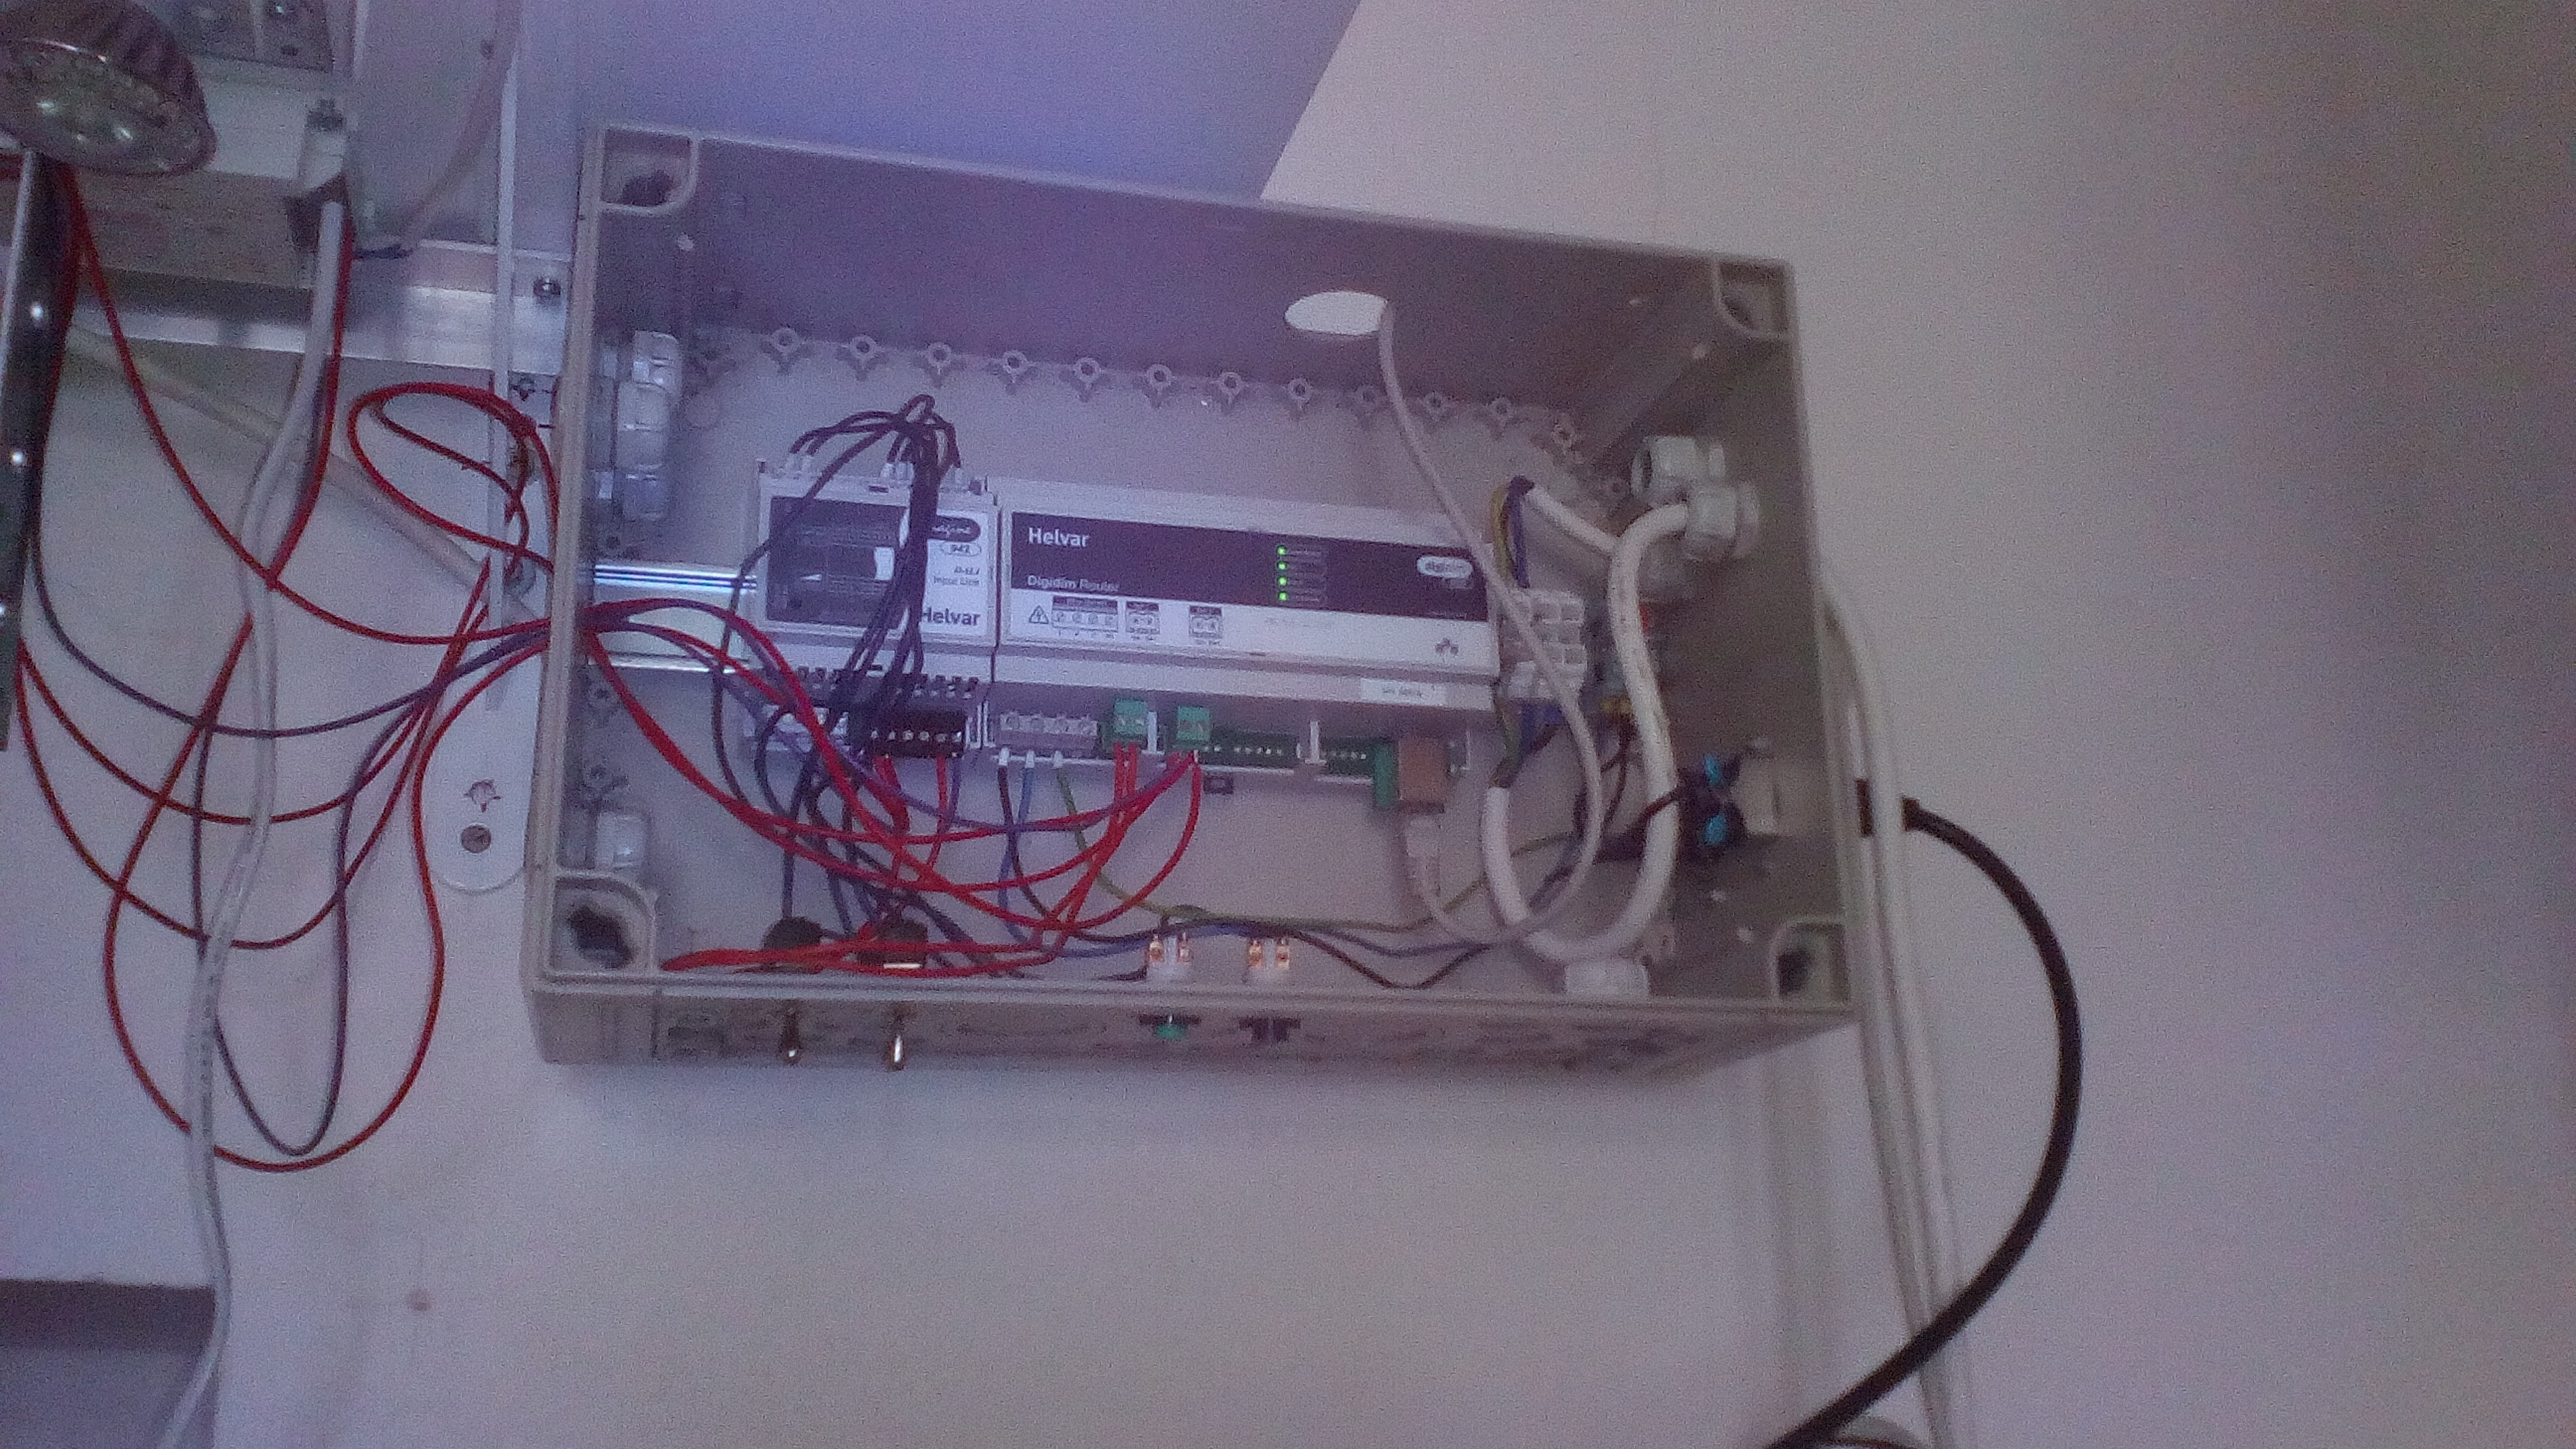
\includegraphics[scale=0.12]{dalisys.jpg}
    		\caption{Dali Digidim Router}
    		\label{dalisys}
    	\end{center}
    \end{figure}
    
    
  \chapter {Měření spotřeby na zářivce}
   Měřením spotřeby se začalo po úspěšném osvojení možností, které systém DALI posky
   tuje. Před samotným měřením se ověřila funkčnost veškerých použitých zařízení včetně počítače a také správnost zapojení samotného obvodu. Zářivka se žhavícími elektrodami, která se k měření využila, pracuje na principu ionizaci rtuťových par při průchodu elektrického proudu a část dodané elektrické energie se přemění na neviditelné ultrafialové záření. Vnitřní stěny trubice zářivky mají tenkou vrstvu luminoforu, který toto záření přemění na viditelné světlo.
   
   \begin{figure}[h]
   	\begin{center}
   			\hspace*{-13mm}
   		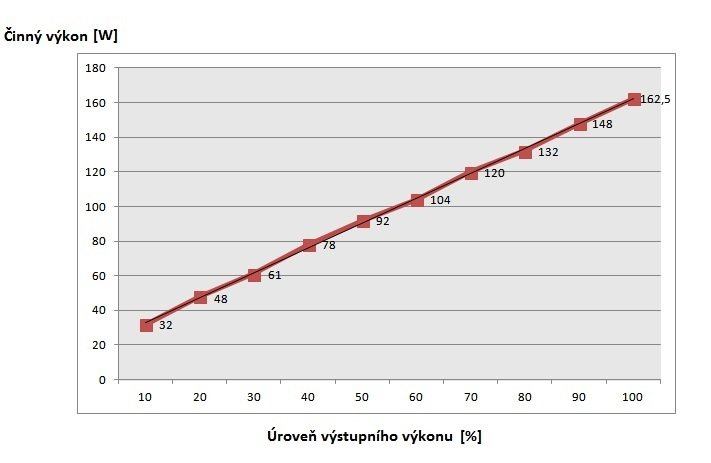
\includegraphics[scale=0.90]{CinnyVyk.jpg}
   		\caption{Průběh činného výkonu}
   		\label{Činík}
   	\end{center}
   \end{figure}
   \section{Popis měření} 
   Se začátkem měřením se začlo nejprve s
   činným výkonem u zářivky, pomocí Wattmetru - obr. \ref{watamp}a připojeného dle schématu na obr. \ref{Scheme}, který bylo třeba přepínat na větší rozsah při vyšších výkonech zářivky, aby nedošlo k  přetížení, a také se zapojením druhého měřícího přístroje, Ampérmetru - obr.  \ref{watamp}b, na zjištění velikosti protékajícího proudu, poté jsem připojil i kleštový ampérmetr, pro změření proudu se musel vodič, kterým protéká proud několikrát namotat pro vysokou přesnost měření, pro měření činného výkonu toto nebylo třeba, poslední, kontrolní měření proběhlo připojením oscilátoru mezi počítač a napojením na obvod, což umožnilo sledovat průběh funkce na počítači. Na obr. \ref{Činík} lze vidět lineárně vzrůstající hodnoty činného výkonu v závislosti na výši jasu, který se zjišťoval postupným zvyšováním intenzity osvětlení přes počítač skrz protokol DALI a odečítáním z displeje obou zmíněných měřáků, zároveň jsem si získané údaje zapisoval do sešitu pro vypočítání dalších nezbytných veličin(Zdánlivý výkon, Účiník). Maximální hodnota 162,5 W celkem odpovídala  udávanému příkonu na zářivce (160 W) .
   
   \begin{figure}[h]
   	\begin{center}
   		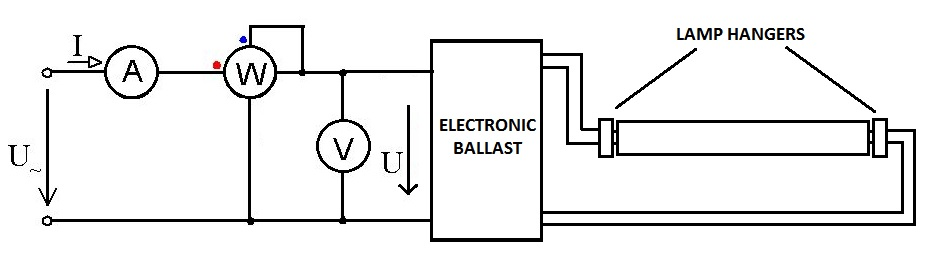
\includegraphics[scale=0.60]{Scheme.jpg}
   		\caption{Schéma zapojení}
   		\label{Scheme}
   	\end{center}
   \end{figure}
    
   
    
  \subsection {Ověření hodnot}
        Ověřování hodnot probíhalo v rámci měření, kdy se sledovala hodnota na dvou měřících jednotkách a porovnávala se mezi sebou, dále se také nahlíželo na hodnoty činného výkonu z programu Helvar Designer, které však nebyly zcela korektní, jak jsem opakovaným měřením zjišťoval. Hodnoty se celkem nelišily, rozdíly byly v řádech procent. 
        
         
        U nízkých hodnot osvětlení byla vypočtena malá hodnota účiníku, která se vzrůstající intenzitou osvětlení zvyšovala, to mě vedlo k zamyšlení, zda nevzniká v systému nějaký úbytek napětí, údaje z osciloskopou podezření potvrdily, Srovnáním těchto údajů lze vidět rušivé vlivy zapříčiňující menší efektivitu světelného zařízení, jak je zřejmé z obr. \ref{bal10} na rozdíl od téměř hladkého průběhu napětí při výši jasu na 50 procentech - viz obr. \ref{bal50}. Projevy rušení byly znát i na hodnotách vypočítaného účiníku - obr. \ref{Účiník} 
 
    \begin{figure}[htp]
    	\begin{center}
    	\subfloat[Wattmetr]{%
    		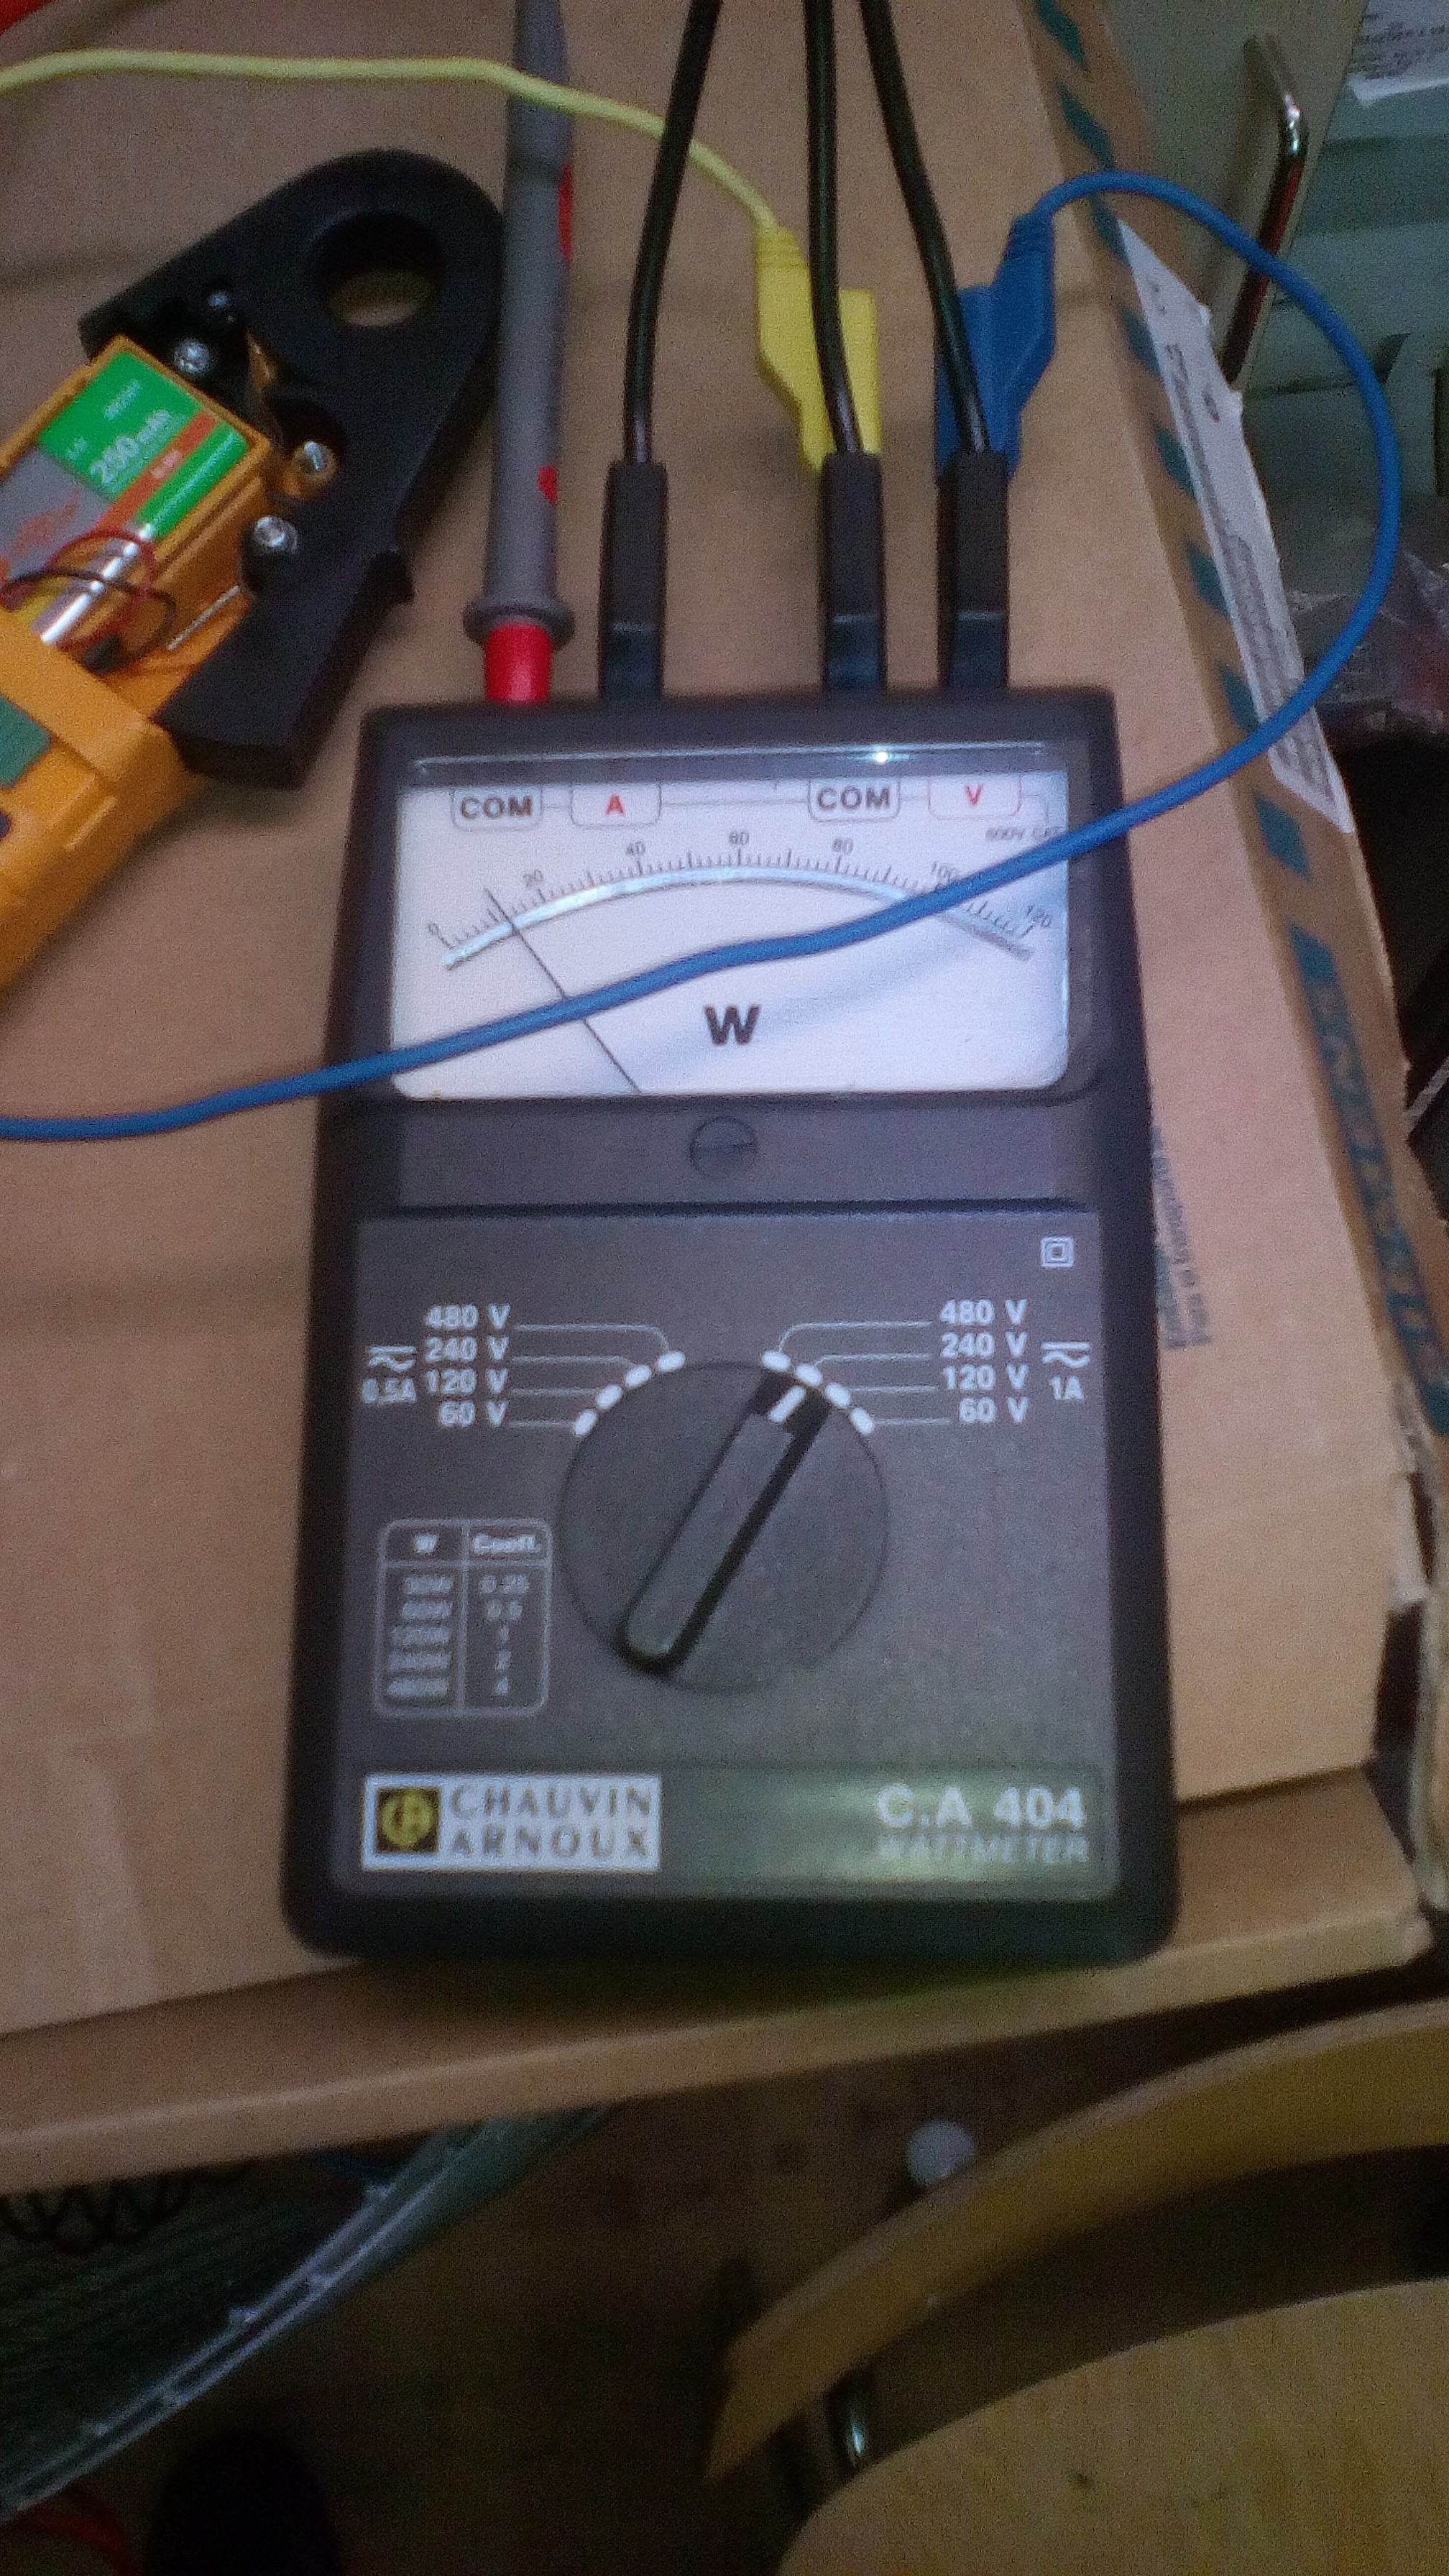
\includegraphics[clip,width=0.4\columnwidth]{wattmer.jpg}%
    	}
    	
    	\subfloat[Ampermetr]{%
    		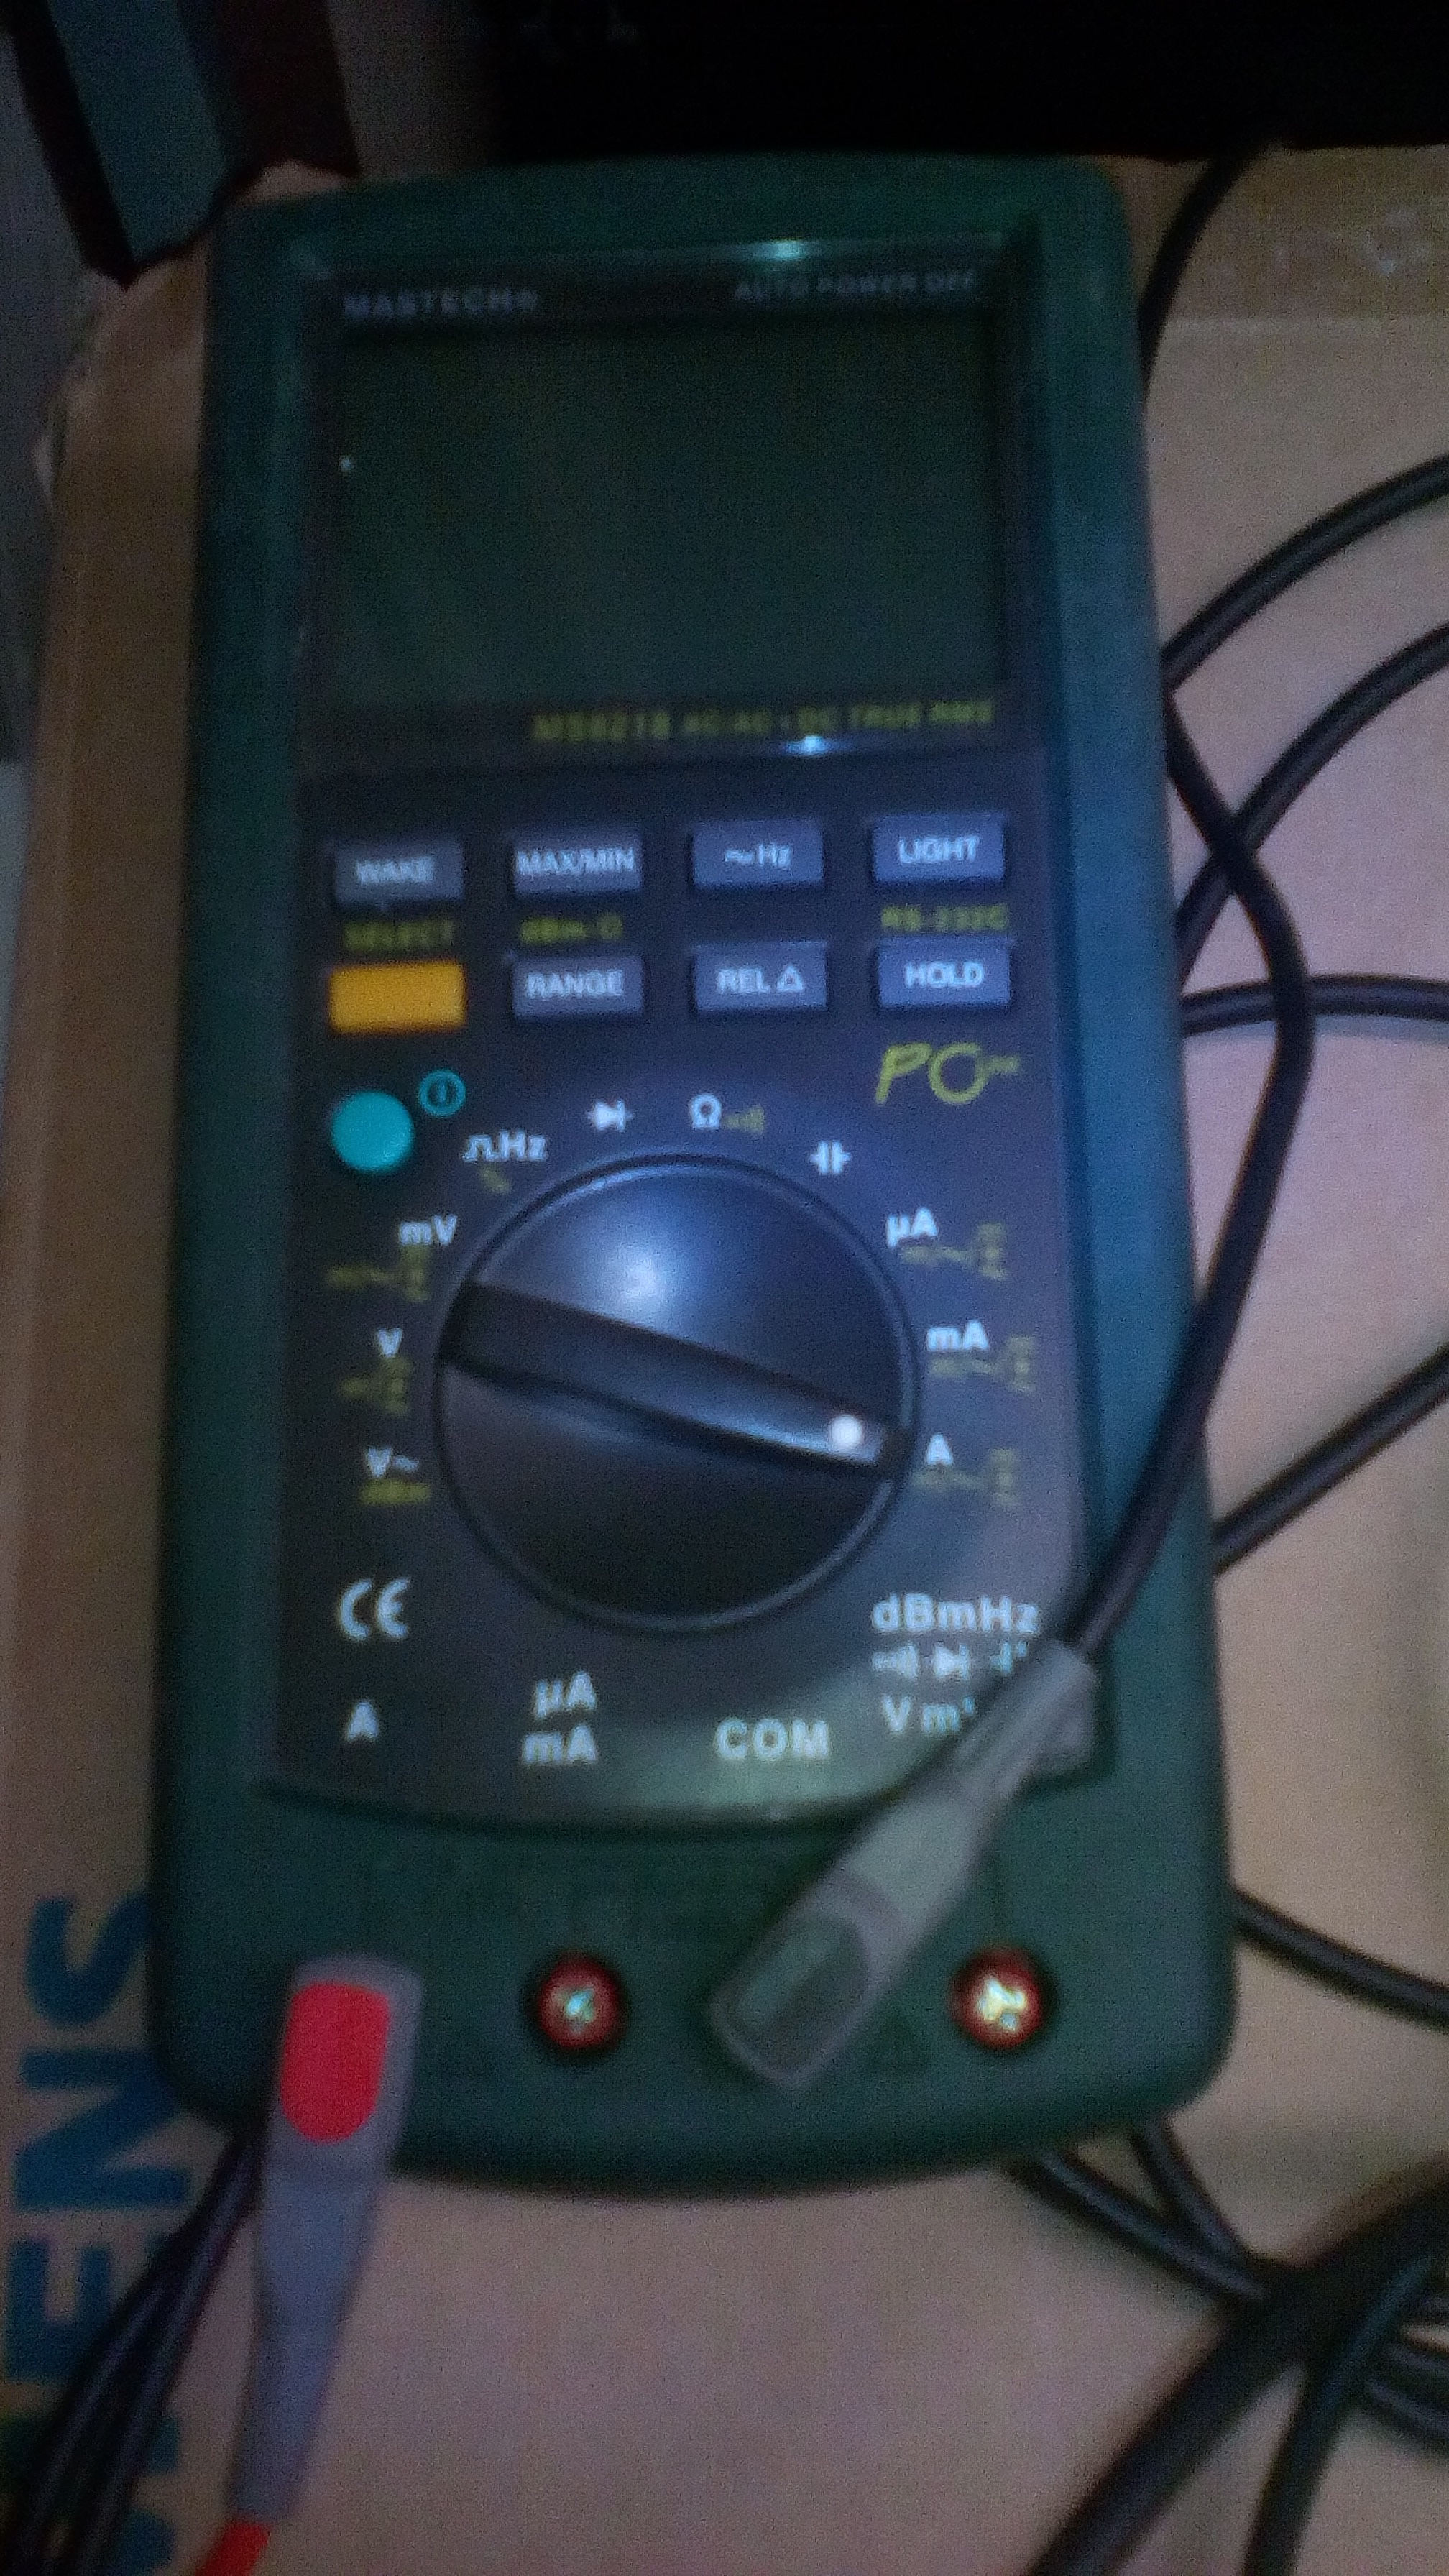
\includegraphics[clip,width=0.4\columnwidth]{ampermetr.jpg}%
    	}
    	
    	\caption{Zapojení wattmetru a ampérmetru}
    	\label{watamp}
   \end{center}	
    \end{figure}
     
 
 
     \begin{figure}[h]
     	\begin{center}
     		\hspace*{-15mm}
     		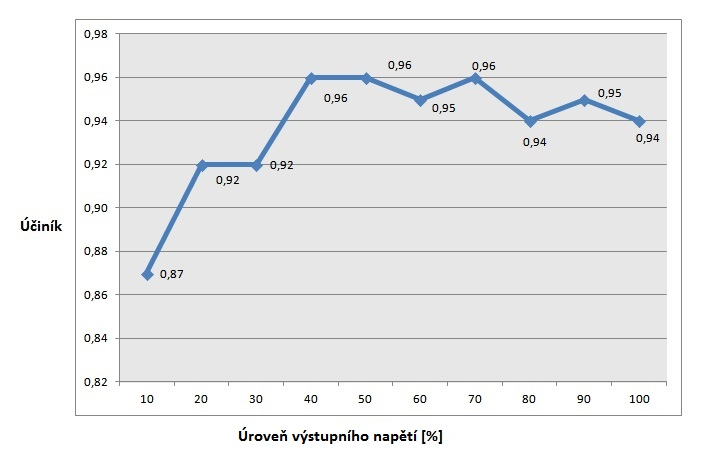
\includegraphics[scale=0.80]{Ucinik.jpg}
     		\caption{Průběh účiníku}
     		\label{Účiník}
     	\end{center}
     \end{figure} 
 
  \section{Výsledky měření}
    Seznámením se s prostředí,m ve kterém se dá pracovat s DALI, jeho ovládáním a celkovým propojením mi umožnilo lépe pochopit chod světelných systémů a umožnilo si prakticky vyzkoušet měření samotné spotřeby na jednom ze světelných zařízení. Efektivita využití při měření byla dosti velká, ztrát se dosáhlo pouze při nízkém osvětlení, což způsobilo deformaci průběhu napětí a ovlivnilo hodnoty účiníku, který byly nízké. Hodnoty proudu tímto způsobem však ovlivněny příliš nebyly. 
     
  \section{Realita} 
   Srovnáním získaných výsledků jsem zjistil, že hodnoty změřeného činného výkonu a protékajícího proudu odpovídaly realitě vzhledem k již zmíněnému lineárnímu průběhu se současnou kontrolou více měřáky naráz. Hodnoty poskytnuté předřadníkem byly mírně zkreslené a mírně zavádějící, lišily se od naměřených hodnot v řádu desítek procent. Deformace průběhu napětí také značí věrohodnost, kdy se mnohdy stane, že dané zařízení se nechová vždy dle očekávání (s minimálním rušením).   
  \vspace{2em}
     \begin{figure}[h]
  	\begin{center}
  		\includegraphics[scale=0.29]{ballast20procent.jpg}
  		\caption{Průběh napětí při úrovni 20 procent jasu} 
  		\label{bal10}
  	\end{center}
  \end{figure}
  
  \begin{figure}[h]
  	\begin{center}
  		\includegraphics[scale=0.29]{ballast50procent.jpg}
  		\caption{Průběh napětí při úrovni 50 procent jasu} 
  		\label{bal50}
  	\end{center}
  \end{figure}
  
  
   \chapter{Závěr}
      Cílem mé práce bylo prozkoumání ovládání světel za pomoci protokolu DALI společně s měřením spotřeby. Seznámení se systémem DALI mi umožnilo vyzkoušet si práci se světelnými zařízeními, což ve výsledku koresponduje s praktickým řízením světel ve firmách.
      
      
      S programem Helvar Designer se mi povedlo naučit se základní funkce řízení světel přes pouhé osvětlení místnosti až po rozsvěcování při detekci pohybu, chvíli trvalo porozumět různým nastavením a jejich významu, ale nakonec přišly kýžené výsledky. Po strávení většiny času s tímto programem jsem se rozhodnul pro měření pouze na jediném svítidle, konkrétně zářivce z důvodu časové tísně.
           
      Patřičné prostudování principů měření jednotlivých výkonů, mi umožnilo vrhnout se s chutí na praktickou část. Zapojením obvodu pro měření veškerých podstatných veličin jsem se dobral ke kýženému měření. Přístroje, se kterými jsem měřil mě nezklamaly a umožnily mi změřit potřebné údaje. Ve výsledku jsem zjistil, že žárovka se chová lineárně, ale jako každé zařízení měla své vady, kdy při menším výkonu vykazovala vyšší ztráty. 
       
      Zpracováním této práce jsem si dokázal, že jsem schopen zvládnout i něco nového a neznámého a rozšířit si mé obzory v oblasti zapojování elektrických obvodů a komunikace se světelnými zařízeními.
      
      
      
      
      
   
  
  
  
\bibliographystyle{unsrt}
\bibliography{test}
\end{document}